\documentclass{article}

%%% Fill details here (in the second brackets)
\newcommand{\name}{Weijie Gan}     % Your name (First Last)
\newcommand{\wustlkey}{gan.weijie}             % Your WUSTL Key
%%%



%%%%%%%%%%%%%%%%%%%%%% Formatting Stuff %%%%%%%%%%%%%%%%%%%%%%%%%%%
\usepackage{times}
\usepackage[T1]{fontenc}

\setlength{\parskip}{1em}\setlength{\parindent}{0pt}
\linespread{1.25}
\usepackage[margin=0.7in,top=1in]{geometry}\usepackage{fancyhdr}
\pagestyle{fancy}\lhead{\bf \name}\rhead{\bf \wustlkey}\cfoot{\thepage}
\newcommand{\info}{\clearpage \subsection*{Information}}
\newcommand{\solution}[1]{\clearpage \subsection*{Solution #1}}
\newcommand{\spart}[1]{\paragraph{(#1)}}
%%%%%%%%%%%%%%%%%%%%%%%%%%%%%%%%%%%%%%%%%%%%%%%%%%%%%%%%%%%%%%%%%%%


%%% Add any more packages if you want to
\usepackage{amsmath,graphicx}


\begin{document} 
%%%%% Main Body goes here

% Begin solution to every problem like this.
\solution{1} 

\spart{a}
The projection function in the first camera is: $p = K[I|\overline{0}] P$, 
where $p = \begin{bmatrix}
  x \\ y \\ 1
\end{bmatrix}$ is camera point and $P = \begin{bmatrix}
  X \\ Y \\ Z \\ 1
\end{bmatrix}$ is world point.

$$
  \begin{bmatrix}
    x \\ y \\ 1
  \end{bmatrix} = \begin{bmatrix}
    f & 0 & 0 \\ 0 & f & 0 \\ 0 & 0 & 1 \\
  \end{bmatrix}\begin{bmatrix}
    1 & 0 & 0 & 0 \\
    0 & 1 & 0 & 0 \\
    0 & 0 & 1 & 0 \\
  \end{bmatrix}\begin{bmatrix}
    X \\ Y \\ Z \\ 1
  \end{bmatrix} = \begin{bmatrix}
    f & 0 & 0 \\
    0 & f & 0 \\
    0 & 0 & 1 \\
  \end{bmatrix}\begin{bmatrix}
    X \\ Y \\ Z
  \end{bmatrix} = \begin{bmatrix}
    fX \\ fY \\ Z
  \end{bmatrix} = \begin{bmatrix}
    \frac{fX}{Z} \\ \frac{fY}{Z} \\ 1
  \end{bmatrix} 
$$

So, $x = \frac{fX}{Z}$.

The projection function in the second camera is: $p' = K[I|t] P$, 
where $p' = \begin{bmatrix}
  x' \\ y' \\ 1
\end{bmatrix}$ is camera point and $P = \begin{bmatrix}
  X \\ Y \\ Z \\ 1
\end{bmatrix}$ is the same world point.

$$
  \begin{bmatrix}
    x' \\ y' \\ 1
  \end{bmatrix} = \begin{bmatrix}
    f & 0 & 0 \\ 0 & f & 0 \\ 0 & 0 & 1 \\
  \end{bmatrix}\begin{bmatrix}
    1 & 0 & 0 & -t_x \\
    0 & 1 & 0 & 0 \\
    0 & 0 & 1 & 0 \\
  \end{bmatrix}\begin{bmatrix}
    X \\ Y \\ Z \\ 1
  \end{bmatrix} = \begin{bmatrix}
    f & 0 & 0 \\
    0 & f & 0 \\
    0 & 0 & 1 \\
  \end{bmatrix}\begin{bmatrix}
    X - t_x \\ Y \\ Z
  \end{bmatrix} = \begin{bmatrix}
    f(X-t_x) \\ fY \\ Z
  \end{bmatrix} = \begin{bmatrix}
    \frac{f(X-t_x)}{Z} \\ \frac{fY}{Z} \\ 1
  \end{bmatrix} 
$$

So, $x' = \frac{f(X-t_x)}{Z}$.

Then, $d = x - x' = \frac{fX}{Z} - \frac{f(X-t_x)}{Z} = 
\frac{fX}{Z} - \frac{fX}{Z} + \frac{ft_x}{Z} = \frac{ft_x}{Z}$

\spart{b}

Based on the above solution:

$$
  \begin{bmatrix}
    x \\ y \\ 1
  \end{bmatrix} =  \begin{bmatrix}
    \frac{fX}{Z} \\ \frac{fY}{Z} \\ 1
  \end{bmatrix} 
$$

which indicates $X = \frac{xZ}{f}$ and $Y = \frac{yZ}{f}$.

We can reexpress $X\alpha + Y\beta + Z\gamma = k$ as:

$$
  \begin{aligned}
    X\alpha + Y\beta + Z\gamma & = k \\
    \frac{xZ}{f}\alpha + \frac{yZ}{f}\beta + Z\gamma & = k \\
    Z (\frac{x}{f}\alpha + \frac{y}{f}\beta + \gamma & ) = k \\
    \frac{1}{k} (\frac{x}{f}\alpha + \frac{y}{f}\beta + \gamma & ) = \frac{1}{Z} \\
  \end{aligned}
$$

Since $d =  \frac{ft_x}{Z}$,

$$
  \begin{aligned}
    ft_x \bigg ( \frac{1}{k} (\frac{x}{f}\alpha + \frac{y}{f}\beta + \gamma & ) \bigg )= d \\
    \frac{\alpha t_x}{k}x + \frac{\beta t_x}{k}y + \frac{fxt_x\gamma}{k} & = d \\
  \end{aligned}
$$

In conclusion, $$\begin{cases}
    a & = \frac{\alpha t_x}{k} \\
    b & = \frac{\beta t_x}{k} \\
    c & = \frac{fxt_x\gamma}{k} \\
\end{cases}$$.

\spart{c}

From $
\begin{bmatrix}
  x \\ y \\ 1
\end{bmatrix} = \begin{bmatrix}
  \frac{fX}{Z} \\ \frac{fY}{Z} \\ 1
\end{bmatrix} 
$, we can get $fX = xZ$ and $fY = yZ$.

$$
  \begin{bmatrix}
    x' \\ y' \\ 1
  \end{bmatrix} = \begin{bmatrix}
    f & 0 & 0 \\ 0 & f & 0 \\ 0 & 0 & 1 \\
  \end{bmatrix}\begin{bmatrix}
    1 & 0 & 0 & 0 \\
    0 & 1 & 0 & 0 \\
    0 & 0 & 1 & -t_z \\
  \end{bmatrix}\begin{bmatrix}
    X \\ Y \\ Z \\ 1
  \end{bmatrix} = \begin{bmatrix}
    f & 0 & 0 \\
    0 & f & 0 \\
    0 & 0 & 1 \\
  \end{bmatrix}\begin{bmatrix}
    X \\ Y \\ Z - t_z
  \end{bmatrix} = \begin{bmatrix}
    fX \\ fY \\ Z - t_z
  \end{bmatrix} = \begin{bmatrix}
    \frac{fX}{Z-t_z} \\ \frac{fY}{Z-t_z} \\ 1
  \end{bmatrix} 
$$

Then $
  x' = \frac{fX}{Z-t_z} = \frac{xZ}{Z-t_z} 
$ and $$
\begin{aligned}
  x'Z-x't_z & = xZ \\
  x' & = \frac{x}{1-\frac{t_z}{Z}} \\
\end{aligned}
$$

Also, $y' = \frac{fY}{Z-t_z} = \frac{yZ}{Z-t_z}$ and $$
\begin{aligned}
  y'Z-y't_z & = yZ \\
  y' & = \frac{y}{1-\frac{t_z}{Z}} \\
\end{aligned}
$$

When $Z \to +\infty$, the co-ordinates $(x', y')$ can match $(x, y)$.

\solution{2} 

\spart{a} Result is shown as figure [\ref{fig:prb2a}].

\begin{figure*}[!h]
  \centering
  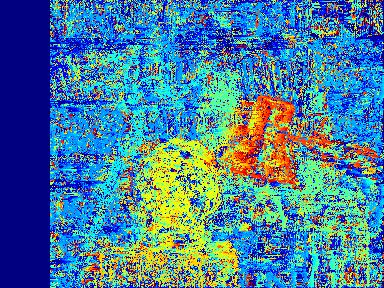
\includegraphics[height=8cm]{code/outputs/prob2a.jpg}
  \caption{Result of Problem 2. (a)}
  \label{fig:prb2a}
\end{figure*}

\spart{b} Result is shown as figure [\ref{fig:prb2b}].

\begin{figure*}[!h]
  \centering
  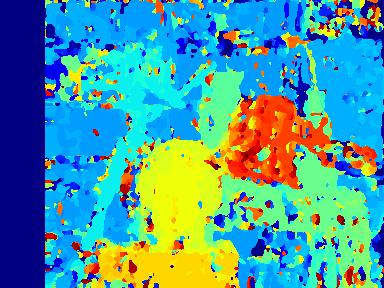
\includegraphics[height=8cm]{code/outputs/prob2b.jpg}
  \caption{Result of Problem 2. (b)}
  \label{fig:prb2b}
\end{figure*}

\solution{3} 

\spart{a} Result is shown as figure [\ref{fig:prb3a}].

\begin{figure*}[!h]
  \centering
  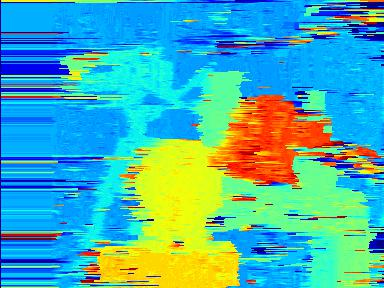
\includegraphics[height=8cm]{code/outputs/prob3a.jpg}
  \caption{Result of Problem 3. (a)}
  \label{fig:prb3a}
\end{figure*}

\spart{b} Result is shown as figure [\ref{fig:prb3b}].

\begin{figure*}[!h]
  \centering
  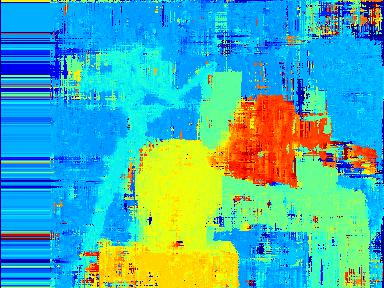
\includegraphics[height=8cm]{code/outputs/prob3b.jpg}
  \caption{Result of Problem 3. (b)}
  \label{fig:prb3b}
\end{figure*}

\solution{4} 

Result is shown as figure [\ref{fig:prb4}].

\begin{figure*}[!h]
  \centering
  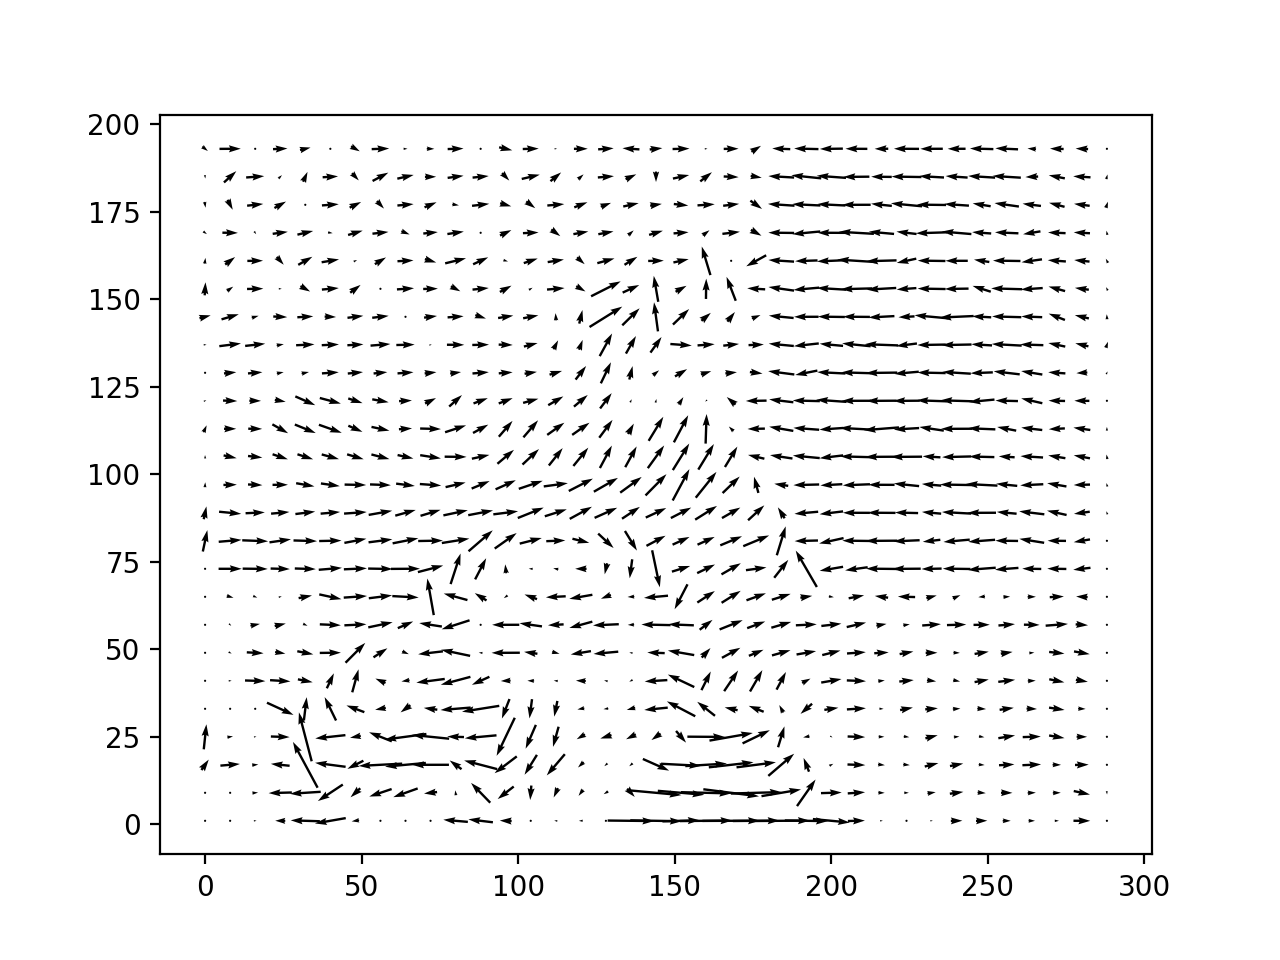
\includegraphics[height=13cm]{code/outputs/prob4.png}
  \caption{Result of Problem 4}
  \label{fig:prb4}
\end{figure*}

%%%%%%%%%% Important, you must edit and complete the informational
%%%%%%%%%% section below. If you discussed the problem set with no
%%%%%%%%%% one, edit it to say no discussions or external resources.
\info

This problem set took approximately 15 hours of effort.

I discussed this problem set with:
\begin{itemize}
  \item I ask one of the classmate for help about prob3a in the class, but I don't know his name. He just sat behind me. 
  I studied the basic idea of how to solve problem and write the code for him. But I did not refer his code.

\end{itemize}

% Note that you might have to escape some special symbols in URLS like \_
% I also got hints from the following sources:
% \begin{itemize}
% \item Wikipedia article on matrix calculus at https://en.wikipedia.org/wiki/Matrix\_calculus
% \item Read numpy tutorial from https://docs.scipy.org/doc/numpy-1.13.0/user/basics.broadcasting.html
% \end{itemize}

\end{document}
